\subsection{Multi-Stage Ensemble}

\begin{figure}[!h]
  \caption{5-fold CV stacked generalization ensemble}
  \centering
    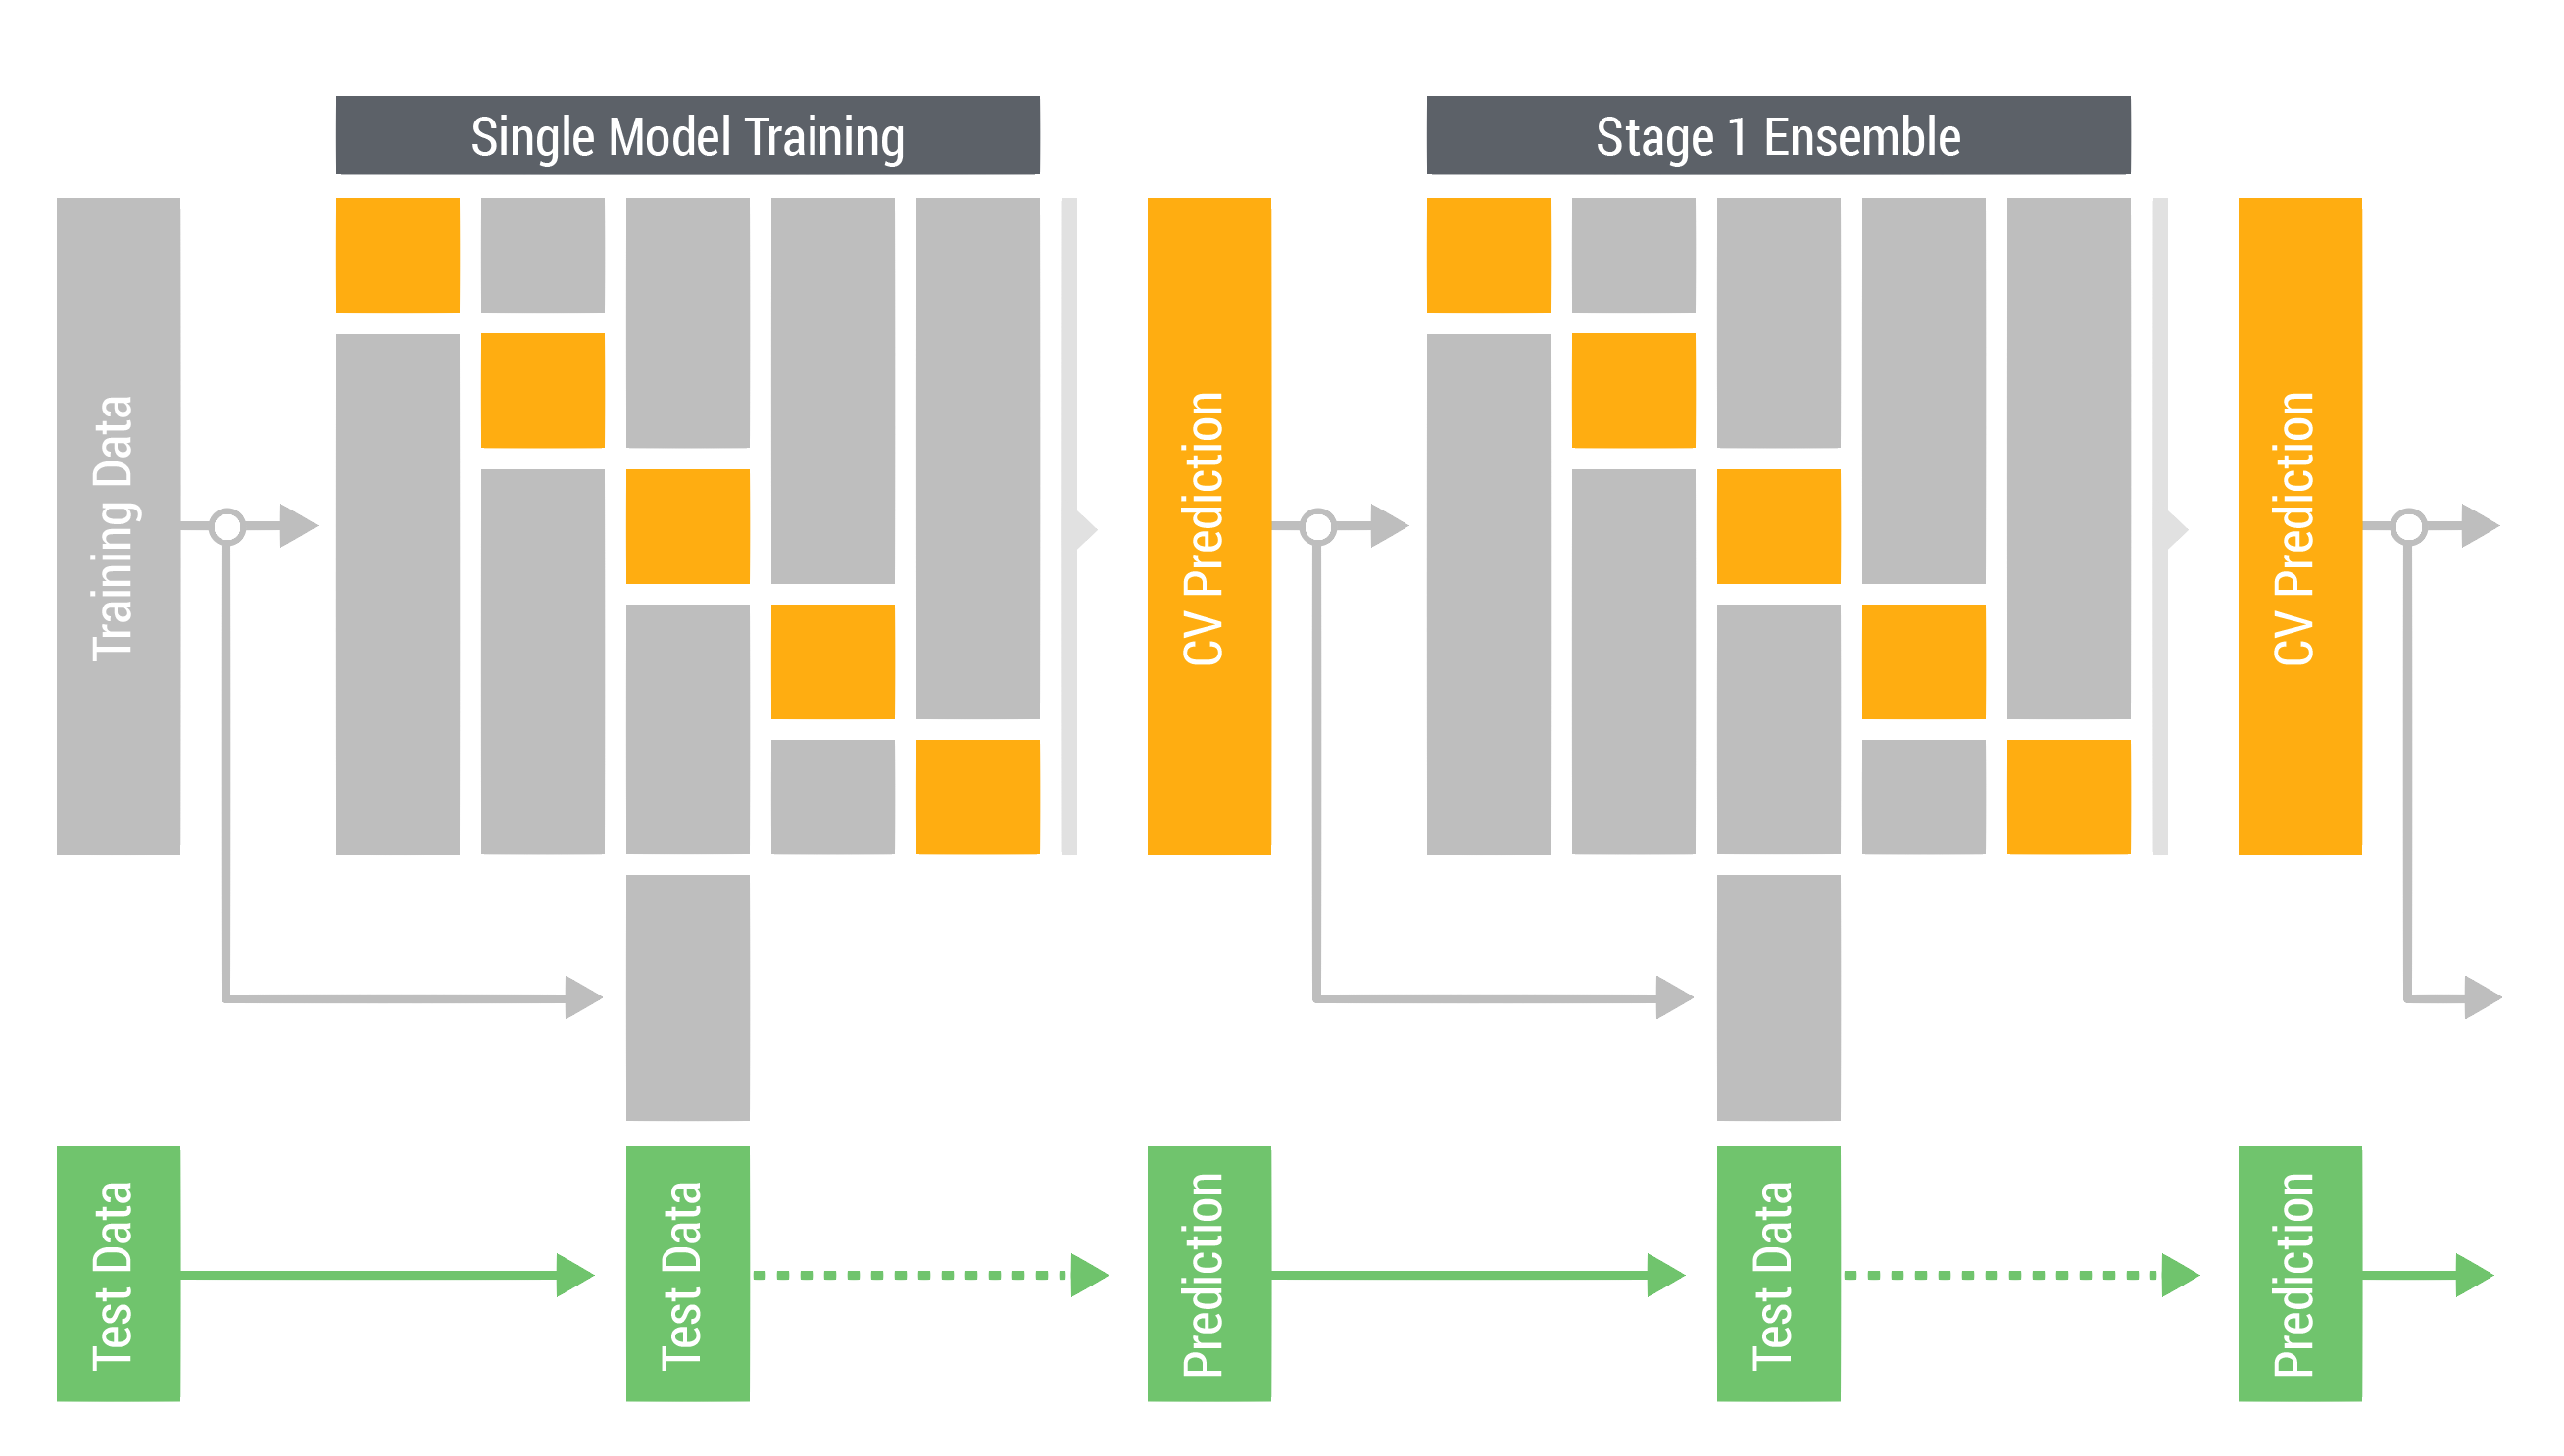
\includegraphics[width=0.5 \textwidth]{cv_ensemble}
\end{figure}

We use the multi-stage ensemble with stacked generalization \cite{wolpert1992stacked, ting1999issues} to blend predictions of multiple models.  As shown in Figure 2, in each stage, we train ensemble models with 5-fold CV, and use the CV and test predictions of models in the previous stage as inputs.  Then, we pass the CV and test predictions of the ensemble models to the next stage as inputs.\\


%final ensemble:
%Read 1|5  trn.final.90788  acc:0.887135  AUC:0.907878
%Read 2|5  esb58v5+magic.dae+nn.validCV.0.907567  acc:0.887143  AUC:0.907567
%Read 3|5  et_esb58v5_rank.val.0.906207  acc:0.886919  AUC:0.906207
%Read 4|5  lr_forward_0.01_esb.esb15v3.val.yht  acc:0.887276  AUC:0.907968
%Read 5|5  xgb_rf.ko_new_feat.txt.valCV.0.906721  acc:0.886753  AUC:0.906721
%linear weights:
%w0=1.96267 w1=0.787138 w2=0.458095 w3=1.61461 w4=1.1703
%final train errors:
%acc:0.887334 AUC:0.908072
%by adding course correction factors AUC on train improved to 0.908194

%Finally we ended up with linear ensembling with 39 courseID correction factors.
%These 39 factors improved the score from 0.90910 to 0.90918.